% 2007 年江西卷理科第 18 题：y=2cos(ωx+θ) 的图象、点 A(π/2,0)、P 与 PA 中点 Q。
%   图中按 θ=π/6、ω=2 及 Q=(2π/3,√3/2)、P=(5π/6,√3) 的示意位置绘制。
% 来源 PDF：gaokaomath-src/普通高考/2007/2007江西理.pdf
% SHA-256：6602cbc393b02e9940beb0035be6e2a28d88a77e0e7792260dcd4c873b542a82
% 原页：2007江西理.pdf 第 1 页（A3 三栏）第 3 栏，书页码 385。
% 重绘依据：按原页余弦曲线、A、P、Q 的相对位置重绘。
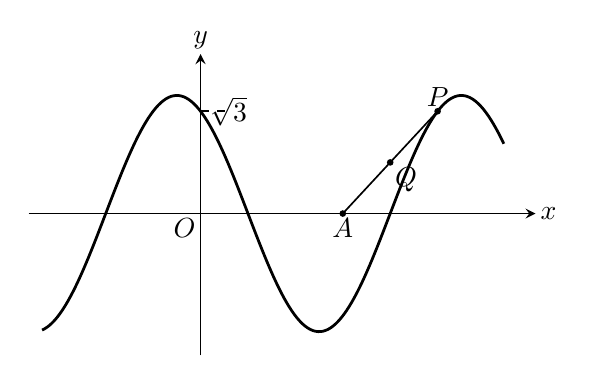
\begin{tikzpicture}[x=1.15cm, y=0.75cm, semithick,
  every node/.style={inner sep=1.5pt}]

  \draw[->,>=stealth] (-1.9,0) -- (3.7,0) node[right] {$x$};
  \draw[->,>=stealth] (0,-2.4) -- (0,2.7) node[above] {$y$};
  \node[below left] at (0,0) {$O$};

  \draw[domain=-1.75:3.35,samples=180,line width=1pt]
    plot (\x,{2*cos(deg(2*\x + pi/6))});

  \coordinate (A) at (1.5708,0);
  \coordinate (Q) at (2.0944,0.8660);
  \coordinate (P) at (2.6180,1.7320);

  \draw (A) -- (P);
  \fill (A) circle (1.2pt);
  \fill (Q) circle (1.2pt);
  \fill (P) circle (1.2pt);
  \node[below] at (A) {$A$};
  \node[below right] at (Q) {$Q$};
  \node[above] at (P) {$P$};

  % y 轴上的 √3 标记
  \draw[dashed] (0,1.732) -- (0.35,1.732);
  \node[right] at (0.05,1.732) {$\sqrt3$};
\end{tikzpicture}
